\documentclass[a4paper,12pt]{article}
\usepackage{t1enc}
\usepackage[longnamesfirst, round]{natbib}  % Bindet den natbib-standard fuer das Zitieren ein
\usepackage{epsfig}
\usepackage[latin1]{inputenc}   % Ermoeglicht Sonderzeichen direkt einzugeben
\usepackage[T1]{fontenc}        % Garantiert saubere Worttrennung bei Umlauten etc.
\usepackage{color}              % Farbpaket
\usepackage{amsmath,amsfonts,amssymb}   % ermoeglicht mathematische Sonderzeichen
\usepackage{ngerman}           % neue deutsche Rechtschreibung
\usepackage[english]{babel}     %
\usepackage{ae}                 %
\usepackage{graphicx}           % Ermoeglicht das Einbinden von Bildern in allen Formaten
\usepackage{longtable}          % zum erstellen von Tabellen ber mehrere Seiten
\usepackage{multirow}           % zum Verbinden von Zeilen innerhalb einer Tabelle
%\usepackage{pictexwd}           % PicTex, ein Graphikpaket
%\usepackage{pst-all, multido}   % psTricks, ein Graphikpaket
\usepackage{url}



% ________________ EINRICHTEN DES DOKUMENTS ______________________%

\bibliographystyle{plainnat}    % legt den Stil fuer das Inhaltsverzeichnis fest

\oddsidemargin 0.1in \evensidemargin 0.1in \textwidth 15.5cm \topmargin -0.4in \textheight 24.5cm
\parindent 0cm      % legt die Seitenraender fest

\pagestyle{plain}          % leere Kopfzeile, Seitennummer in der Mitte der Fusszeile

\newcommand{\bs}{\boldsymbol}  % shortcut zur Erzeugung von fetten Sympolen in der Mathe-Umgebung

\renewcommand{\baselinestretch}{1.25}
% 1,5 -facher Zeilenabstand (Standard ist 1,2-facher Zeilenabstand, also 1,2*1,25 = 1,5



\begin{document}

% ________________ TITELSEITE ______________________%


\pagenumbering{roman}   % roemische Zahlen zur Seitennumerierung

\begin{titlepage}       % Umgebung fuer Titelseite, frei gestaltbar

\thispagestyle{empty}   % keine Numerierung auf Titelseite


\begin{center}
\vspace*{2.5cm}
{\bf  \Large The Distribution of Wealth \\in a Life-Cycle Model with Durables} \\
\vspace*{3cm} 
Master Thesis \\ in Economics \\
Prof. Dr. Thomas Hintermaier  \\
\vspace*{0.5cm} 
Summer Term 2017\\
\end{center}

\vfill
\begin{flushright}
   \emph{Eric Lustenberger} \\
    \emph{Heckenweg 38}\\
    \emph{3007 Bern}\\
   \emph{Student Number}\\
 \emph{Economics}\\

\end{flushright}



% 
% \begin{center}
% $ $			% oeffnet und schliesst eine Matheumgebung (Trick, um den Titel nach unten zu rutschen
% \vspace{4cm}
% 
% {\LARGE TITEL}
% \vskip 4cm
% 
% Diese Seite ist frei gestaltbar
% \end{center}

\end{titlepage}

\newpage                % erzwingt an dieser Stelle einen Seitenumbruch



% ________________ INHALTSVERZEICHNIS ______________________%


% \tableofcontents   %fuegt Automatisch ein Inhaltsverzeichnis ein
% 
% \newpage
% 


% ________________ HAUPTTEIL ______________________%


\pagenumbering{arabic}      % Seitenzahlen wieder arabisch numerieren
\setcounter{page}{1}        % Ruecksetzen des Seitenzahlzaehlers auf 1


\section{\"Introduction}
\label{Chapter1}

\subsection{Unter\"Uberschrift}

\subsubsection*{UnterUnter\"Uberschrift}



Hier steht mal ein Text. Eine M\"oglichkeit des Zitierens ist, direkt
im Text die Quelle anzugeben \citep[see][pp.225-369]{key1}.
Andererseits schreiben \cite{key2}, dass man auch so zitieren kann.

In der Matheumgebung kann der oben (im Latex-Quellcode) genannte Shortcut verwendet
werden, um aus einem normalen $\beta$ ein fettes $\bs \beta$ zu
machen. Wichtige Gleichungen, die nochmal verwendet werden, sollten nummeriert werden, z.B.
\begin{equation}
\label{eq:ols}
   b = (x'x)x'y \;.
\end{equation}

Nebens\"achlicheres, auf das man sich nicht mehr bezieht, bleibt unnummeriert, also 
\begin{equation*}
   a = 1\;.
\end{equation*}
Nun kann man direkt auf die erste Gleichung als Gleichung~\eqref{eq:ols} verweisen mittels des zugewiesenen labels. In gleicher Weise kann man auf die Graphik~\ref{fig:ersteGraphik} bzw. Graphik~\ref{fig:andereGraphik} verweisen. Die Tilde zwischen \glqq Graphik\grqq{} und \glqq \verb|\ref{fig:andereGraphik}|\grqq{} verhindert, dass bei Zeilenumbr\"uchen die Zahl als erstes alleine in die neue Zeile rutscht. Ganz analog f\"ur die Tabelle~\ref{tab:Tabelle}. 



\section{Ben\"otigte Programme}

unter Windows:
\begin{itemize}
   \item Miktex (\url{http://miktex.org/})
   \item ein Editor, je nach Geschmack z.B. WinEdt (\url{http://www.winedt.com/}; kostenpflichtige Studentenversion) oder einen der vielen anderen verf\"ugbaren, z.B. TeXnicCenter (\url{www.texniccenter.org/})
   \item ghostview und ghostscript (\url{http://pages.cs.wisc.edu/~ghost/}
\end{itemize}
unter Linux:
\begin{itemize}
   \item Latex ist in den meisten Verteilungen enthalten, z.B. tetex in Suse (ggf. \"uber yast nachinstallieren)
   \item als Editor empfiehlt sich z.B. Kile
\end{itemize}
f\"ur die Literatur:\\
z.B. JabRef (\url{http://jabref.sourceforge.net/})


\section{Pr\"asentationen}

Beispiele f\"ur Pr\"asentationen mit dem Beamer-Style:

\url{http://www.informatik.uni-freiburg.de/~frank/latex-kurs/latex-kurs-3/Latex-Kurs-3.html}


\section{Literature Overview}
\label{Chapter2}

Investigate empirical predictions of the life-cycle incomplete markets model (\cite{Gourinchas&Parker2002}; \cite{cagetti2003}; \cite{castaneda2003}; \cite{yang2009}; \cite{kaplan2010}; \cite{hintermaier2011}), thus contribute to the literature that (note copy paste.... demonstrate that a plausibly parameterized version of their models can quantitatively explain empirical findings as arising from rational choices of consumers facing an increasing wage profile and income uncertainty.)
The model is based on the classic income-fluctuation problem in which the consumer faces a stochastic income process and decides in every period how much to save and how much to consume. Important contributions to the literature are Deaton (1991), Carroll (1992,1997), \cite{Gourinchas&Parker2002}. (note copy paste... Following Bewley (1986), this problem has been embedded by Huggett (1993) and Aiyagari (1994) into a general equilibrium framework, giving rise to the endogenous determination of the interest rate as well as a nontrivial income, wealth, and consumption distribution at equilibrium.)
(Note copy paste... Furthermore, this paper relates to other literature such as: 
Endogenous borrowing constraint: The specification of the borrowing constraint  in \cite{FV&K2011} is adapted from the recent endogenous incomplete-markets literature: Kehoe and Levine (1993), Kocherlakota (1996), Krueger and Perri (1999, 2006), and Alvarez and Jermann (2000). Lustig (2004) also has a model with durable assets and an endogenous borrowing constraint to explain the equity premium puzzle, however agents have full access to Arrow securities and are infinitely lived.
Literature on optimal portfolio choice in the presence of consumer durables: Grossman and Laroque (1990), Eberly (1994), Chah et al. (1995), and Flavin and Yamashita (2002).)

Note: missing citations, not all of the above are cited properly!!!!!

Literature on wealth distribution!!!!! 

\section{The Life-Cycle Model}
\label{Chapter3}
In the following section I discuss the economic model considered and outline the most important considerations made within the literature. Firstly, I discuss the life-cycle modeling and the literature, which applies life-cycle and to be more exact imperfect markets models in the context of wealth distributions. Secondly, I present my modeling choices and solution methods applied for this particular problem. 
\subsection{Modeling Literature}

\subsection{The Model}
Before going into a more detailed description of the model at hand it is important to understand the modelling choice. Why a life-cycle model with an imperfect market structure? Why include durables as an  additional asset choice to the more standard approach, which does summarize all assets in a one period bond, such as for example \cite{hintermaier2011}? 

To answer the first question I will mainly refer to the the literature. The second will be discussed in a more detailed manner in the following section, which treads the life-cycle profiles and especially the importance of modeling durables. 

\subsubsection{Imperfect market structure}
The choice of an exogenously determined imperfect market structure allows for a straight forward answer. It comes down to the economic question one poses. The aim here is to demonstrate that such a model can quantitatively explain the empirical net-wealth distribution in the US. The role the imperfect market structure, entering as a limited choice of assets to fully insure against idiosyncratic wage shocks, poses, is thus to produce an endogenous wealth distribution. The savings are fist and foremost driven by a precautionary motive to insure for future wage shocks. Knowing that the income may drop in the future consumers save today to achieve a more stable consumption across their live. In a complete market framework consumers could perfectly diversify away idiosyncratic risks \citep{a&w2010}  (and thus would not build a buffer stock of savings for future shocks.) (???????? is this exact?????)
The hypothesis of the complete market framework has been rejected by the vast majority of empirical research \citep{a&w2010}. \cite{deaton1994} show that the life cycle profile of consumption inequality is increasing with age, a fact that would be inconsistent with complete markets. Moreover, the assuming away markets, where individuals can trade contingent claims to insure themselfs against the idiosyncratic wage shocks is justified by moral hazard problems \citep{FV&K2011}. While in some rare cases - such as when only studying aggregates, it may still be sufficient to consider a complete market framework, when considering wealth-distributive questions, the imperfect market assumption is both necessary from a theoretical perspective and well-founded from an empirical perspective. It remains to discuss the whether it makes sens to treat distributive issues from a life-cycle point of view.

\subsubsection{Life-Cycle}

As \cite{deaton1994} show, consumption inequality seems to vary with age. Further empirical research does support these findings, indicating that some of the differences in earnings, income, and wealth across households can be attributed to differences in the household's age \cite{rios2016} (FIND BETTER REFERENCES?). \cite{hintermaier2011} Show that the average net-wealth increases with wealth and that the dispersion of wealth falls with age. 
Moreover, there is a vast theoretical literature using a different versions of the life-cycle model to discuss distributive questions.  \cite{Gourinchas&Parker2002}; \cite{cagetti2003}; \cite{castaneda2003}; \cite{yang2009}; \cite{kaplan2010};\cite{hintermaier2011} (CITE MORE RECENT LITERATURE!!!)
while there are also some that use infinite horizon models....

Finally, the choice to study the empirical validity of a life-cycle model, which produces a net-wealth distribution arising from rational choices of consumers subject to income uncertainty, moreover allows for a detailed analysis of consumption and savings behavior over a person's live-cycle. A coherent framework incorporating the behavior of household's over their lifespan is paramount for the study of re-distributive policies. (Cite....)
These factors thus support the choice of a life-cycle model. 


\subsubsection{Partial Equilibrium}
Last but not least, partial equilibrium as modeling choice has to be discussed briefly. (????????????????)

(copy paste from hintermaier 2011
Note that we assume that changes in the domestic supply of assets do not affect do not affect the interest rate. As in a small-open economy, this price is determined exogenously (on the world markets.) \footnote{This assumption is not restrictive for our purposes since we observe the price in our ex post analysis for the period 1983-2007. Hence, the supply of assets and the observed price suffice to determine the equilibrium asset quantities. This allows us to be agnostic about the price elasticity of asset demand.})



\subsubsection{Consumer's Problem}
As established above, the baseline model in question is a life-cycle model with an imperfect market structure. I closely follow \cite{hintermaier2010}.\footnote{In order to facilitate comparability, I will closely follow the notation used in their paper.} While there algorithm allows for both a live-cycle and infinite-horizon models, the example model presented in their paper uses the latter. For reasons discussed above, I will in this case opt for a live-cycle formulation. Finally, the baseline model does not include adjustment costs. These are considered in a later section of the model. 

There is a continuum of risk averse consumers with a finite time horizon. 
At age 90 consumers die with certainty, younger consumers between the age of 26 and 90 may die with probability $\pi_{j} < 1$ at age $j$. Until retirement the labor income of each individual $i$ $y_{ij}$ is stochastic. After the age 65 is completed, they retire with certainty and receive individual-specific retirement benefits $b_{i}$.\footnote{The construction of these benefits is discussed in the Appendix.}
Consumers derive utility from a durable good $d$ and a non-durable good $c$. The utility function $U(c,d)$ is strictly concave, increasing and non-separable in c and d (REALLY??? When not??? all three true???). 
In each period consumption $c_{j}$, the durable good $d_{j+1}$ and the financial risk-free asset $a_{j+1}$ are chosen after receiving the income. Agents then derive utility from consumption and durable services, before the assets pay returns. While the liquid assets return an interest rate $r$ durables depreciate at rate $delta$. As previously discussed, such a market structure implies that markets are incomplete and agents will accumulate a buffer stock in order to save for rainy days. The ex-ante identical consumers thus will thus, depending on their income trajectory, end up with different portfolios of the endogenous state variables. The model is therefore suited to match empirical facts about net worth positions since it does produce an endogenous distribution of portfolios, which differs in age and income. Moreover, (THE ADVANTAGE OF DURABLES) besides providing services and thus allowing consumers to derive utility from durables, their durability implies, that they may be used as collateral. It is assumed that all credit needs to be collateralized.\footnote{About 85\% of household debt in the Survey of Consumer Finances 2004 is secured by collateral.\citep{hintermaier2010}} 
\\
The collateral constraint takes the form:

\begin{equation}
\underbrace{\mu(1-\delta)d_{j+1} + \gamma\underline{y}}_{collateral} \geq -(1+r)a_{j+1}
\end{equation}

where $\underline{y}$ is the minimum labor income realization \footnote{CHECK THIS WITH CODE!!!} and $\mu \in [0,1) and \gamma \in [0,1)$ are the respective fractions of the durable stock and of minimum labor income, which can be collateralized.
\footnote{It is important to note that this constraint guarantees full repayment by consumers and thus acts as non-bankruptcy constraint. This is assured by the timing assumptions made above \textendash The lender does know the financial portfolio choice $(a_{j+1},d_{j+1})$ and the minimum of the support of the income distribution $\underline{y}$, however future individual income draws $y_{j+1}$ do remain obscure to him. Finally, note that only choices in $j$ determine, whether the constraint is binding or not. }

It is useful to rewrite the constraint in terms of total wealth and future durable holdings. Total wealth available to a consumer in each period is 

\begin{equation}
x_{j} \equiv (1+r)a_{j} + (1-\delta)d_{j},
\end{equation}

rewritten the constraint then looks like this:

\begin{equation}
x_{j+1} \geq -\gamma\underline{y}+(1-\mu)(1-\delta)d_{j+1}
\end{equation}

One now sees that total wealth needs to be larger than the negative value of the minimum fraction of income that can be collateralized and the fraction of wealth which cannot be used as collateral. Furthermore, under the assumption that $\mu < 1$ $d_{j+1}$ is determined for a given $x_{j+1}$, when the constraint binds.

Although in my baseline model they are set to 0, I also consider the case where durables can only be adjusted with some costs: 

\begin{equation}
\Psi(d_{t+1},d_{t})=\frac{\alpha}{2}\left(\frac{d_{t+1}-(1-\delta)d_{t}}{d_{t}}\right)^2d_{t}.
\end{equation}\footnote{\citep{hintermaier2010} use the same specification, which is based on the investment literature (COPY PASTE(see, for example, \cite{adda2003dynamics},p.192)). Costs are differntiable in $d_{t+1}$ and $d_{t}$. Moreover, by letting the durable stock depreciate, consumers can avoid these costs. In this particular specification, adjustment costs do not affect the collateral constraint, as it is assumed that these costs do not have an impact on the sales of collateral seized by lenders. NOTE \citep{hintermaier2010} EXPLAIN IN APPENDIX VERSION WHERE THIS IS THE CASE.}

Finally, the specification of the budget constraint, follows from the above:

\begin{equation}
a_{j+1}+d_{j+1}+c_{j}+\Psi(d_{t+1},d_{t})=x_{j}+y_{j}
\end{equation}



\paragraph{The recursive formulation of the household problem} 

I will proceed by depicting the case prior to retirement. (SPECIFY RETIREMENT CASE!!!)
We let $T^{r}$ denote the first period of retirement.
The Bellman equation prior to retirement, if  $j < T^{r}$thus is:

\begin{equation}
v_{j}(x_{j},d_{j},y_{j}) = \max_{\substack{a_{j+1},d_{j+1}}}\left[U(\underbrace{x_{j}+y_{j}-a_{j+1}-d_{j+1}-\Psi(d_{t+1},d_{t})}_{c_{j}},d_{j})+\hat{v_{j}}(x_{j+1},d_{j+1},y_{j})\right]
\end{equation}

where the expected next period value function is discouted by the product of the probability of survival $(1-\pi_{j})$ and the discount factor $\beta$
\begin{equation}
\hat{v_{j}}(x_{j+1},d_{j+1},y_{j}) \equiv \beta (1-\pi_{j})E_{j}v_{j+1}(x_{j+1},d_{j+1},y_{j+1}),\textnormal{\footnote{Note that the income $y_{j}$ ensters the expected value of next period's utility function as a state, due to its persistence.}}
\end{equation}



with the constraints: 

\begin{equation}
a_{j+1}+d_{j+1}+c_{j}+\Psi(d_{t+1},d_{t})=x_{j}+y_{j},
\end{equation}

\begin{equation}
x_{j+1} = (1+r)a_{j+1} + (1-\delta)d_{j+1},
\end{equation}

\begin{equation}
x_{j+1} \geq -\gamma\underline{y}+(1-\mu)(1-\delta)d_{j+1}, 
\end{equation} (WHAT HAPPENS WITH MIN Y IN RETIREMENT????)

\begin{equation}
d_{j+1} \geq d_{min},
\end{equation}


FROM RED PAPER HELP TO SPECIFY CASE WITH RETIREMENT!!!
We specify our model in discrete time. Rearranging the budget constraint, consumption of individual $i$ with age $j$ is 

\begin{equation}
c_{ij} = 
  \begin{cases}
    (1+r)a_{i,j-1}-a_{ij}+y_{ij} & \quad \text{if } j < T^{r}, \\
    (1+r)a_{i,j-1}-a_{ij}+b(z_{i,T^{r}-1}) & \quad \text{if } j \geq T^{r},\\
  \end{cases}
\end{equation}

where $b(z_{i,T^{r}-1})$ are the retirement benefits. These benefits depend on the last realization of labor income before retirement $z_{i,T^{r}-1}$ as we explain further in the next section. Defining cash-on-hand as 

\begin{equation}
x_{ij} = 
  \begin{cases}
    (1+r)a_{i,j-1}+y_{ij} & \quad \text{if } j < T^{r}, \\
    (1+r)a_{i,j-1}+b(z_{i,T^{r}-1}) & \quad \text{if } j \geq T^{r},\\
  \end{cases}
\end{equation}

we can write the Bellman equation as 

\begin{equation}
V_{j}(x_{ij},y_{ij})= \max_{ \substack{a_{ij} \geq 0}}[u(\underbrace{x_{ij}-a_{ij}}_{c_{ij}}) + \beta(1-\delta_{j})E_{j}V_{j+1}(x_{i,j+1},y_{i,j+1})],
\end{equation}

where we restrict the choice of assets to $a_{ij} \geq 0$, as motivated in the previous section.)

\subsubsection{Numerical algorithm}

The problem above does not provide a closed-form solution and thus the solution has to be approximated numerically. As already mentioned above, the model is based on \cite{hintermaier2010} and I can therefore directly apply their algorithm. They expand the endogenous gridpoints method (EGM) proposed by \cite{carroll2006} for a problem with two states and thus providing a very efficient algorithm to solve models with durables and collateralized debt. \footnote{Solving such models has been considered particluarly expensive and challenging, as durables enter as additional state (if non-separability utility from durables and non-durable or adjustemnt costs are allowed for) and durables increase the dimensionality of the portfolio choice.\citep{hintermaier2010}} 

(NOTE THAT ALGORITHM MUST BE CHANGED FOR CASE WITH ADJUSTMENT COSTS)

Given the life-time sequences for income (as described in the income process section) {$y_{kj}$} and survival probabilities (CHECK ON HOW TO BEST WRITE DOWN!) {$(1-\pi_{j})$}, $\forall j = 1,...,T $ (AND ALL MARKOV STATES $k$) the algorithm starts with an exogenous grid for the future state $x', G_{x'} \equiv {x'_{1},x'_{2},...,x'_{I}}$, the current state $d, G_{d} \equiv {d_{1},d_{2},...,d_{J}}$.

The algorithm starts iterates recursively over the policy function starting with the last period $j=T$ in which the consumer sells all durables and liquid assets to consume before death. It thus holds that $x'=d'=a'=0$ and thus the initial consumption policy is $c(x,d_{j},y_{kj})=x+y_{j,k}$.For each period t < T-1, the algorithm proceeds as follows. In a first step it maps $x'$ into $d'$ and in a second step it solves for the current choice c and state x from optimal future combinations (x',d'). Moreover, the values for the exogenous grid are chosen such that the results are not affected. (BE MORE PRECISE
INDICATE DIFFERENCES BETWEEN POST/PRE RETIREMENT (expectation)!




NOT NECESSARY FROM HERE ON. HOWEVER MAYBE BE MORE PRECISE ABOVE!


For each period t < T-1, the algorithm proceeds as follows: 

\paragraph{Step 1: Mapping $x'$ into $d'$} 

Using the optimal relationship,
\begin{equation} \label{eq:optimal_algorithm}
\tiny
K_{ijk}\left((1+r)\left(1+\frac{\partial \Psi(d'_{ijk},d_{j})}{\partial d'}\right)-\mu(1-\delta)\right)-\eta_{ijk} = -\left(\frac{\partial \Psi(d'_{ijk},d_{j})}{\partial d'}(1+r)+r+\delta \right) \frac{\partial \hat{v}(x'_{i},d'_{ijk},y_{k})}{\partial x'}+\frac{\partial \hat{v}(x'_{i},d'_{ijk},y_{k})}{\partial d'},
\end{equation}
in the algorithm determines the values of, $d'_{ijk}$ for a given $y_{k}$ and $d_{j}$, which correspond to each of the exogenous gridpoints $x'_{i}$.\footnote{The partial derivatives are obtained by exploiting the envelope conditions. When considering adjustment costs one therefore has to solve for $\partial \Psi(d'',d') /\partial d'$. In the first iteration this is done by making use of terminal condition $d''=0$. For every iteration that follows $d''$ is then replaced by the previously computed optimal policy.(COPY PASTE: Note that with adjustment costs, full decumulation is feasible for all x,d and y if $\mu < 1-(1-\delta)\alpha/2$, which is satisfied for the chosen parameters below!!!!!!!!!!!}

There are three possible cases for each  $y_{k}$ and $d_{j}$, to compute the optimal $d'_{ijk}$.\footnote{Note that the optimal solution necessarily lies in the interval imposed by the collateral constraint and the lower bound on $d'$, $[d_{min},\bar{d_{i}}]$, where $\bar{d_{i}} \equiv \frac{x'_{i}+\gamma \underline{y}}{(1-\mu)(1-\delta}$.}
\paragraph{Case 1 \textendash  Neither the collateral nor the constraint on durables are binding} Hence, $K_{ijk}=\eta_{ijk}=0$ and thus the there exists a $d'_{ijk}$ for which the right hand side of \ref{eq:optimal_algorithm} is 0.
\paragraph{Case 2 \textendash the right hand side of \ref{eq:optimal_algorithm} is positive} jklh
\paragraph{Case 3 \textendash the right hand side of \ref{eq:optimal_algorithm} is negative} lkjg

\paragraph{Step:2 Obtaining current choice c and state x from optimal future combinations (x',d')}

\subsubsection{Comparing the simulation output with SCF data}

\subsubsection{Calibration}

\paragraph{Utility Function}
I consider the same class of preferences as \cite{hintermaier2010}, which is commonly used in the literature considering durable and non-durable consumption (CITE MORE). 

\begin{equation}
U(c,d)=\frac{\psi(c,d)^{1-\sigma}-1}{1-\sigma} \ \ \textnormal{where} \ \ \psi(c,d)=c^{\theta}(d+\epsilon_{d})^{1-\theta}, \ \textnormal{\footnote{The Cobb-Douglas specification is approximately validated by empirical evidence \citep{FV&K2011}}}
\end{equation}

where I assume $\epsilon_{d} > 0$, which thus indicates a number small enough to be irrelevant for the quantitative exercise at hand but nonetheless larger than zero. The utility function thus allows for zero consumption of durables, while the INADA-Condition ensures that people always consume some non-durables, i.e. they cannot survive without food, but are allowed to survive without houses and cars.(NOTE MIGHT LOOK AT DIFFERENCE BETWEEN EQUAL TO ZERO AND NOT EQUAL TO ZERO SINCE HINTERMAIER ALLOWS FOR BOTH(COPY PASTE: Allowing for the potentially optimal choice $d' = d_{min}$ means that the constraint for minimal durable holdings needs to be taken into account in the recursive problem as another occasionally binding constraint in addition to the collateral constraint!!!). 

The utility function thus, is strictly increasing durable consumption and non-durable consumption, strictly concave and obeying the Inada conditions with respect to nondurable consumption. 

\citep{FV&K2011} utility form death is normalized to 0 ??????????

\paragraph{Data (Initializing DATA + probability of death (PLOT!)}

\paragraph{Income Process}

\begin{enumerate}
\item \citep{FV&K2011} stochastic labor income process up to age 65, where they impose mandatory retirement. Differs from other specifications such as Abowd and Card (1989), Carroll (1992), or Gourinchas and Parker (2002) in two aspects: 
\begin{enumerate}
\item do not allow labor income to go to zero- very low probability Carroll (1992) estimates it at 0.003 for a year. However, its effects on the intertemporal allocations are quite big, since hh will not borrow any positive amount since they might face a lifelong sequence of zero labor income and might be unable to consume a positive amount and repay their debt in some period. (Moreover, argument of public income-support programs in the US -> labor in the model is after-tax, after-government transfer labor income.
\item unit root in AR process is not imposed  ( is something that is debated -> they show that their results are not very sensitive toward this issue -> increase $\rho$ toward unity (LOOK AT STORESLETTEN ET AL: (2001) -> do not reject unit root.
\end{enumerate} 
\item Check \cite{hintermaier2010} and \cite{hintermaier2011}
\end{enumerate}

\paragraph{Others NOTE: INCOMPLETE LOOK AT PAPERS}
\begin{enumerate}
\item The interest rate
\begin{enumerate}
\item \citep{FV&K2011} $r = 4\%$(NOTE CITING A WORKING PAPER!!!) \footnote{\citep{mcgrattan2001}}

\item \citep{hintermaier2010} (COPY PASTE: The annual real interest rate is set to 3\% and the depreciation rate is 2\% (see, for example, Caporale and Grier, 2000; Lustig and van Nieuwerburgh, 2005). The low depreciation rate is motivated by the dominating role of housing for consumer durables.
\end{enumerate}
\end{enumerate}

\begin{enumerate}
\item Preference Parameters
\begin{enumerate}
\item  \citep{FV&K2011} $\theta = 0.81$ and $\beta = 0.9375$ matching the ratio of expenditures on nondurables and durables $C/I^{d} = (C/Y)/(I^{d}/Y) = 6.2$, which is the long-run average for U.S. data.

\item \cite{hintermaier2010} choose $\sigma = 0$, commonly used in the literature and then calibrate $\theta$ and $\beta$ to match (up to precision $10^{-2}$) the amount of wealth in total data, 6.33 in terms of average population labor earnings taken after taxes and transfers, and the part of wealth accounted for by durables, 4.45. \footnote{When they compute the statistic in the data, they use sampling weights provided in the SCF. (COPY PASTE: Note that the normalization by net labor and the use of equivalence scales implies that normalized (aggregate) wealth is larger than the wealth to output ratio.)}
\end{enumerate}
\end{enumerate}
\section{Why model durables?}
\begin{enumerate}
\item \cite{FV&K2011} 
\begin{enumerate}
\item empirical observation that durables constitute a large fraction of households' asset holdings - hh hold 35\% of their total assets in durables and only 28\% in equity (flow of funds account 2nd quarter) 
\item the life-cycle pattern of nondurable consumption may be closely related to the life-cycle pattern of the accumulation of durables and thus any abstraction to net wealth may severely bias the study of asset accumulation (and life-cycle profile of nondurable consumption
\end{enumerate}
\end{enumerate}


\section{Life-Cycle Profiles}
As discussed above, the choice of a life-cycle model is mainly motivated by the fact, that age plays an important role in questions related to wealth distribution and in particular to the net-wealth distribution. This section will give insight into the accumulation of wealth by agents over their lifetime. As we will see, this also affects consumption. \cite{FV&K2011} have pointed out that it is paramount to consider durables in order to properly model the life-cycle profile of consumption, which is hump shaped (see . The first section discusses empirical results as well as life-cycle profiles produced by models from theoretical research. In the second section I will produce and comment on the life-cycle profile of my baseline model and then go over to a more detailed investigation of certain factors in the third section. 

\subsection{Life-Cycle profiles in the data and theoretical literature}


\subsection{Profiles predicted by the model}
Averages, in what Units?
\begin{enumerate}
\item \cite{hintermaier2016} averages and in average net labor earning
\item 
\end{enumerate}

\begin{figure}
\caption{Average Consumption over the Life-Cycle} 
\label{cash_equivalent_ue_vs_e}	%label, um spaeter auf die Graphiknummer zugreifen zu koennen
\centering
\includegraphics[scale=.5]{Figures/Consumption_LCP}  % width legt Breite der Graphik fest

\begin{minipage}{0.8\linewidth}
\footnotesize{NEED TO INDICATE THE MEASURES. JUST VERY STANDARD! NEEDS TO BE UPDATED}
\end{minipage}

\end{figure}

\begin{figure}
\caption{Average Income over the Life-Cycle} 
\label{cash_equivalent_ue_vs_e}	%label, um spaeter auf die Graphiknummer zugreifen zu koennen
\centering
\includegraphics[scale=.5]{Figures/Income_LCP}  % width legt Breite der Graphik fest

\begin{minipage}{0.8\linewidth}
\footnotesize{NEED TO INDICATE THE MEASURES. JUST VERY STANDARD! NEEDS TO BE UPDATED}
\end{minipage}

\end{figure}



\begin{figure}
\caption{Average Durable Holdings over the Life-Cycle} 
\label{cash_equivalent_ue_vs_e}	%label, um spaeter auf die Graphiknummer zugreifen zu koennen
\centering
\includegraphics[scale=.5]{Figures/Durables_LCP}  % width legt Breite der Graphik fest

\begin{minipage}{0.8\linewidth}
\footnotesize{NEED TO INDICATE THE MEASURES. JUST VERY STANDARD! NEEDS TO BE UPDATED}
\end{minipage}

\end{figure}

\begin{figure}
\caption{Average Asset Holdings over the Life-Cycle} 
\label{cash_equivalent_ue_vs_e}	%label, um spaeter auf die Graphiknummer zugreifen zu koennen
\centering
\includegraphics[scale=.5]{Figures/Liquid_Assets_LCP}  % width legt Breite der Graphik fest

\begin{minipage}{0.8\linewidth}
\footnotesize{NEED TO INDICATE THE MEASURES. JUST VERY STANDARD! NEEDS TO BE UPDATED}
\end{minipage}

\end{figure}

\begin{figure}
\caption{Average Net Worth over the Life-Cycle} 
\label{cash_equivalent_ue_vs_e}	%label, um spaeter auf die Graphiknummer zugreifen zu koennen
\centering
\includegraphics[scale=.5]{Figures/Net_Worth_LCP}  % width legt Breite der Graphik fest

\begin{minipage}{0.8\linewidth}
\footnotesize{NEED TO INDICATE THE MEASURES. JUST VERY STANDARD! NEEDS TO BE UPDATED}
\end{minipage}

\end{figure}

\subsection{What drives the life-cycle profiles within the model?}

\label{Chapter4}
\section{The Wealth Distribution}
\label{Chapter5}
\section{Conclusion}
\label{Chapter6}
%_________________ ENDE DES HAUPTTEILS_________________%


\newpage


%_________________ Literaturverzeichnis _______________%

\addcontentsline{toc}{section}{References}        % Fuegt im Inhaltsverzeichnis "References" hinzu
\bibliography{bib_thesis}                         % Erstellt Literaturverzeichnis (bindet das file bib_thesis.bib ein

%_________________ Platz fuer Graphiken und Tabellen _______________%

\newpage

% Einfuegen einer Grafik
\begin{figure}
\caption{titel der Graphik} 
\label{fig:ersteGraphik}	%label, um spaeter auf die Graphiknummer zugreifen zu koennen
\centering
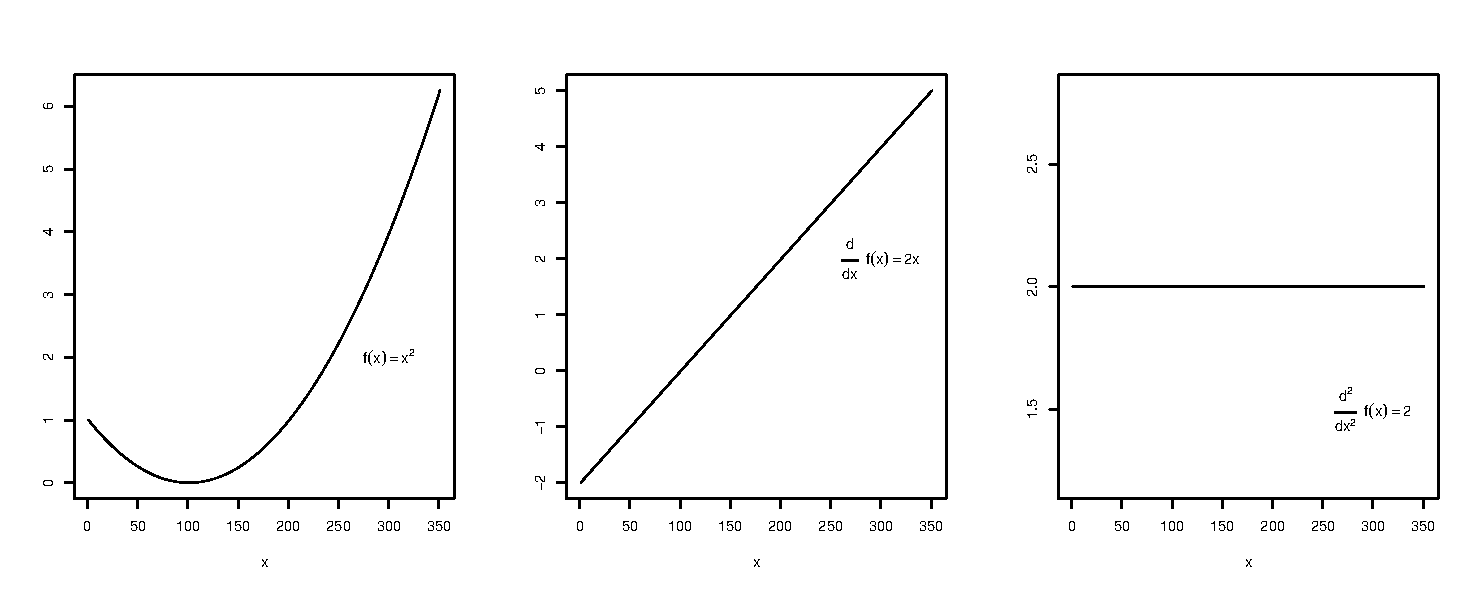
\includegraphics[width=6.5cm]{abb1.png}  % width legt Breite der Graphik fest

\begin{minipage}{0.8\linewidth}
\footnotesize{die Graphik sollte beschrieben werden, sodass man ohne den Text vorne zu lesen wei\ss{}, worum es geht: panel 1 zeigt die Funktion, panel 2 die erste Ableitung und Panel 3 die zweite Ableitung}
\end{minipage}

\end{figure}

\begin{figure}
\caption{titel der Graphik}
\label{fig:andereGraphik} \centering
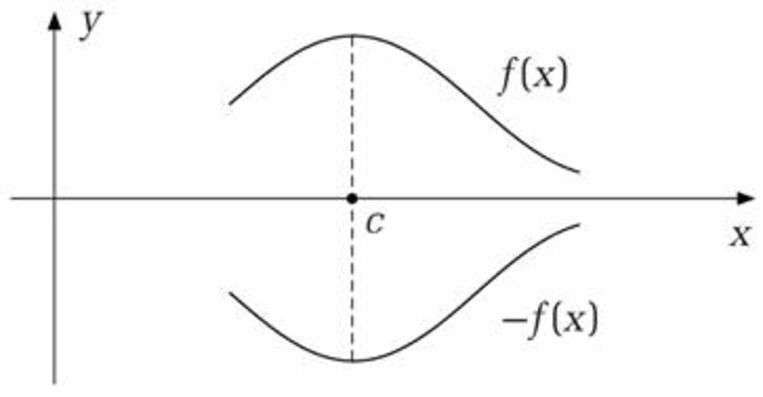
\includegraphics[angle=90,height=6.5cm]{abb2.jpg}  % angle dreht die Graphik, falls noetig; height legt die Hoehe der Graphik fest

\end{figure}

\begin{table}
\caption{Der Title der Tabelle}
\label{tab:Tabelle}
\centering
 \begin{tabular}{lc|r}
   Eine & kleine & Tabelle\\
\hline
   Text links & mittig & oder rechts \\
   & unterstrichen  & \\
\cline{2-2}
   \multicolumn{2}{c|}{\"uber zwei Spalten} & dritte Spalte \\
\end{tabular}   
\end{table}

   





\end{document}
